\chapter{Logic}
\begin{flushright}
\english{The only way to rectify our reasonings is to make them as tangible as those of the Mathematicians, so that we can find our error at a glance, and when there are disputes among persons, we can simply say: Let us calculate [calculemus], without further ado, to see who is right.}\\ --- Leibniz
\end{flushright}
\minitoc

Note:  This chapter is currently very chaotic because of a re-organization effort.  Fuzziness, $\mathcal{Z}$, is no longer considered a foundational part of the logic.

\section{Background}

\subsection{Turing universality}

\subsubsection{Undecidability of FOL.}

\subsection{$\lambda$-calculus}

(See Wikipedia: \href{http://en.wikipedia.org/wiki/Lambda_calculus}{Lambda calculus}).

\subsubsection{Bound variables:}  In the abstraction $(\lambda x.t)$ we call $x$ the bound variable and $t$ the body.  Every occurrence of $x$ in $t$ is \textbf{bound} by the abstraction.  Conversely, an occurrence of a variable $y$ is \textbf{free} if it is not bound, eg in $(\lambda z.(\lambda x.(yx)))$.

\subsubsection{Head-normal form:}  A $\lambda$ term is in head-normal form if, for $m \geq 0$ and $n \geq 0$, it can be expressed as:
$$\lambda x_1 ... x_m . \; x t_1 ... t_n.$$
The variable $x$ may either be free or bound (one of $x_1,...,x_m$).

\subsubsection{De Bruijn indexes.}

\subsubsection{Director strings.}

\subsection{Functional programming}

\subsection{Combinatory logic}

(See Wikipedia: \href{http://en.wikipedia.org/wiki/Combinatory_logic}{Combinatory logic}).

\subsection{Term-rewriting systems}

\subsection{Simple type theory}

\subsection{Higher-order logic}

HOL is roughly synonymous with type theory, with the addition of axioms that define logical primitives.

\subsubsection{Standard semantics and general semantics (of higher-order logic).}

How is Henkin semantics reducible to FOL?

\subsection{Model theory}

Model theory is the study of the truth of syntactic formulas defined via their correspondence to certain mathematical structures known as models.  Originated by Alfred Tarski.

\subsection{Proof theory}

\subsection{Deduction systems}

\subsubsection{Hilbert systems.}

\subsubsection{Sequent calculus.}

\subsubsection{Natural deduction.}

\subsubsection{Tableau.}

\subsubsection{Resolution.}

%\section{Logic and pre-logic}
%
%Designing the perfect logic is nearly impossible, as witnessed by the proliferation of alternative logics in recent decades.  \textbf{Pre-logics}, or logical frameworks, are attempts to reduce logics to simpler computational mechanisms, and thus to tackle the problem in a general way.
%
%The candidates for pre-logics include:
%\begin{compactenum}[\textbullet ]
%\item $\lambda$ calculus
%\item combinatory logic
%\item term-rewriting systems
%\item grammars
%\item programs (such as genetic programs)
%\item etc
%\end{compactenum}
%
%The basic configuration of a system with pre-logic is like this:
%\begin{figure}[H]
%\centering
%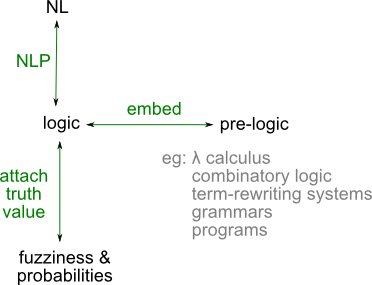
\includegraphics[scale=0.7]{prelogic.png}
%% \caption{Prelogic}
%\end{figure}
%NL should be translated into logic because logic is closer to NL than pre-logic.  What really distinguishes ``logic'' from pre-logic is the notion of \textbf{propositions}, which is a unit of meaning to which we can attach \textbf{truth values}.  A proposition such as \formula{male(john)} is a ``complete'' entity of meaning, as opposed to the predicate \formula{male} which is incomplete, or ``syncategorematic''\footnote{The term syncategorematic has several meanings, here I mean any component of a sentence that is not a proposition.}.  This distinction is important because fuzziness and probabilities should be assigned to the logic rather than pre-logic.
%
%The problem with the above configuration is, if the pre-logic is fixed and the logic is allowed to be dynamically learned, then it may be difficult to work with such a dynamically changing logic, in particular to assign fuzzy-probabilistic truth values to it, or to translate NL to it.

\section{Concept composition}

\subsection{Fragments}

Is it possible to have inference at the sub-propositional level?  Inference rules that operate upon fragments of propositions?  Sometimes our human minds can focus on fragments or concepts that are not complete sentences.

For example, we may think of ``spaghetti with meat balls'' instead of ``spaghetti with meat balls are tasty''.  Or we may think ``To lose more weight, I need to...'' without being able to complete the sentence immediately.

It seems possible to extend the idea of logical inference from propositions to fragments:

\begin{center}
\begin{tabular}{|c|c|}
\hline
\textbf{logic of propositions}   & \textbf{logic of fragments} \\
\hline
$A \rightarrow$ B                     & $\vect{a} \rightarrow \vect{b} $ \\
(implication)                              & (completion and jump) \\
\hline
special/general-ize                    & special/general-ize \\
in subsumption order               & in ontology \\
\hline
$\approx$                                  &  $\approx$ \\
(similarity of formulas)             &  (similarity of fragments) \\
\hline
$\neg A$                                   &  $\overline{\vect{a}}$ \\
(not)                                           & (opposite) \\
\hline
\end{tabular}
\end{center}
\vspace{0.5cm}

\textbf{Completion} means to extend a fragment to become a longer fragment or a complete proposition.

\textbf{Jump} means to jump from a fragment to another fragment or proposition in the KB.

Notice that completion and jump are supported by the KB, in the sense that they draw information from the KB in order to ``push'' through the arrow, just like in deduction.  The following figure illustrates their similarity:
\begin{figure}[H]
\centering
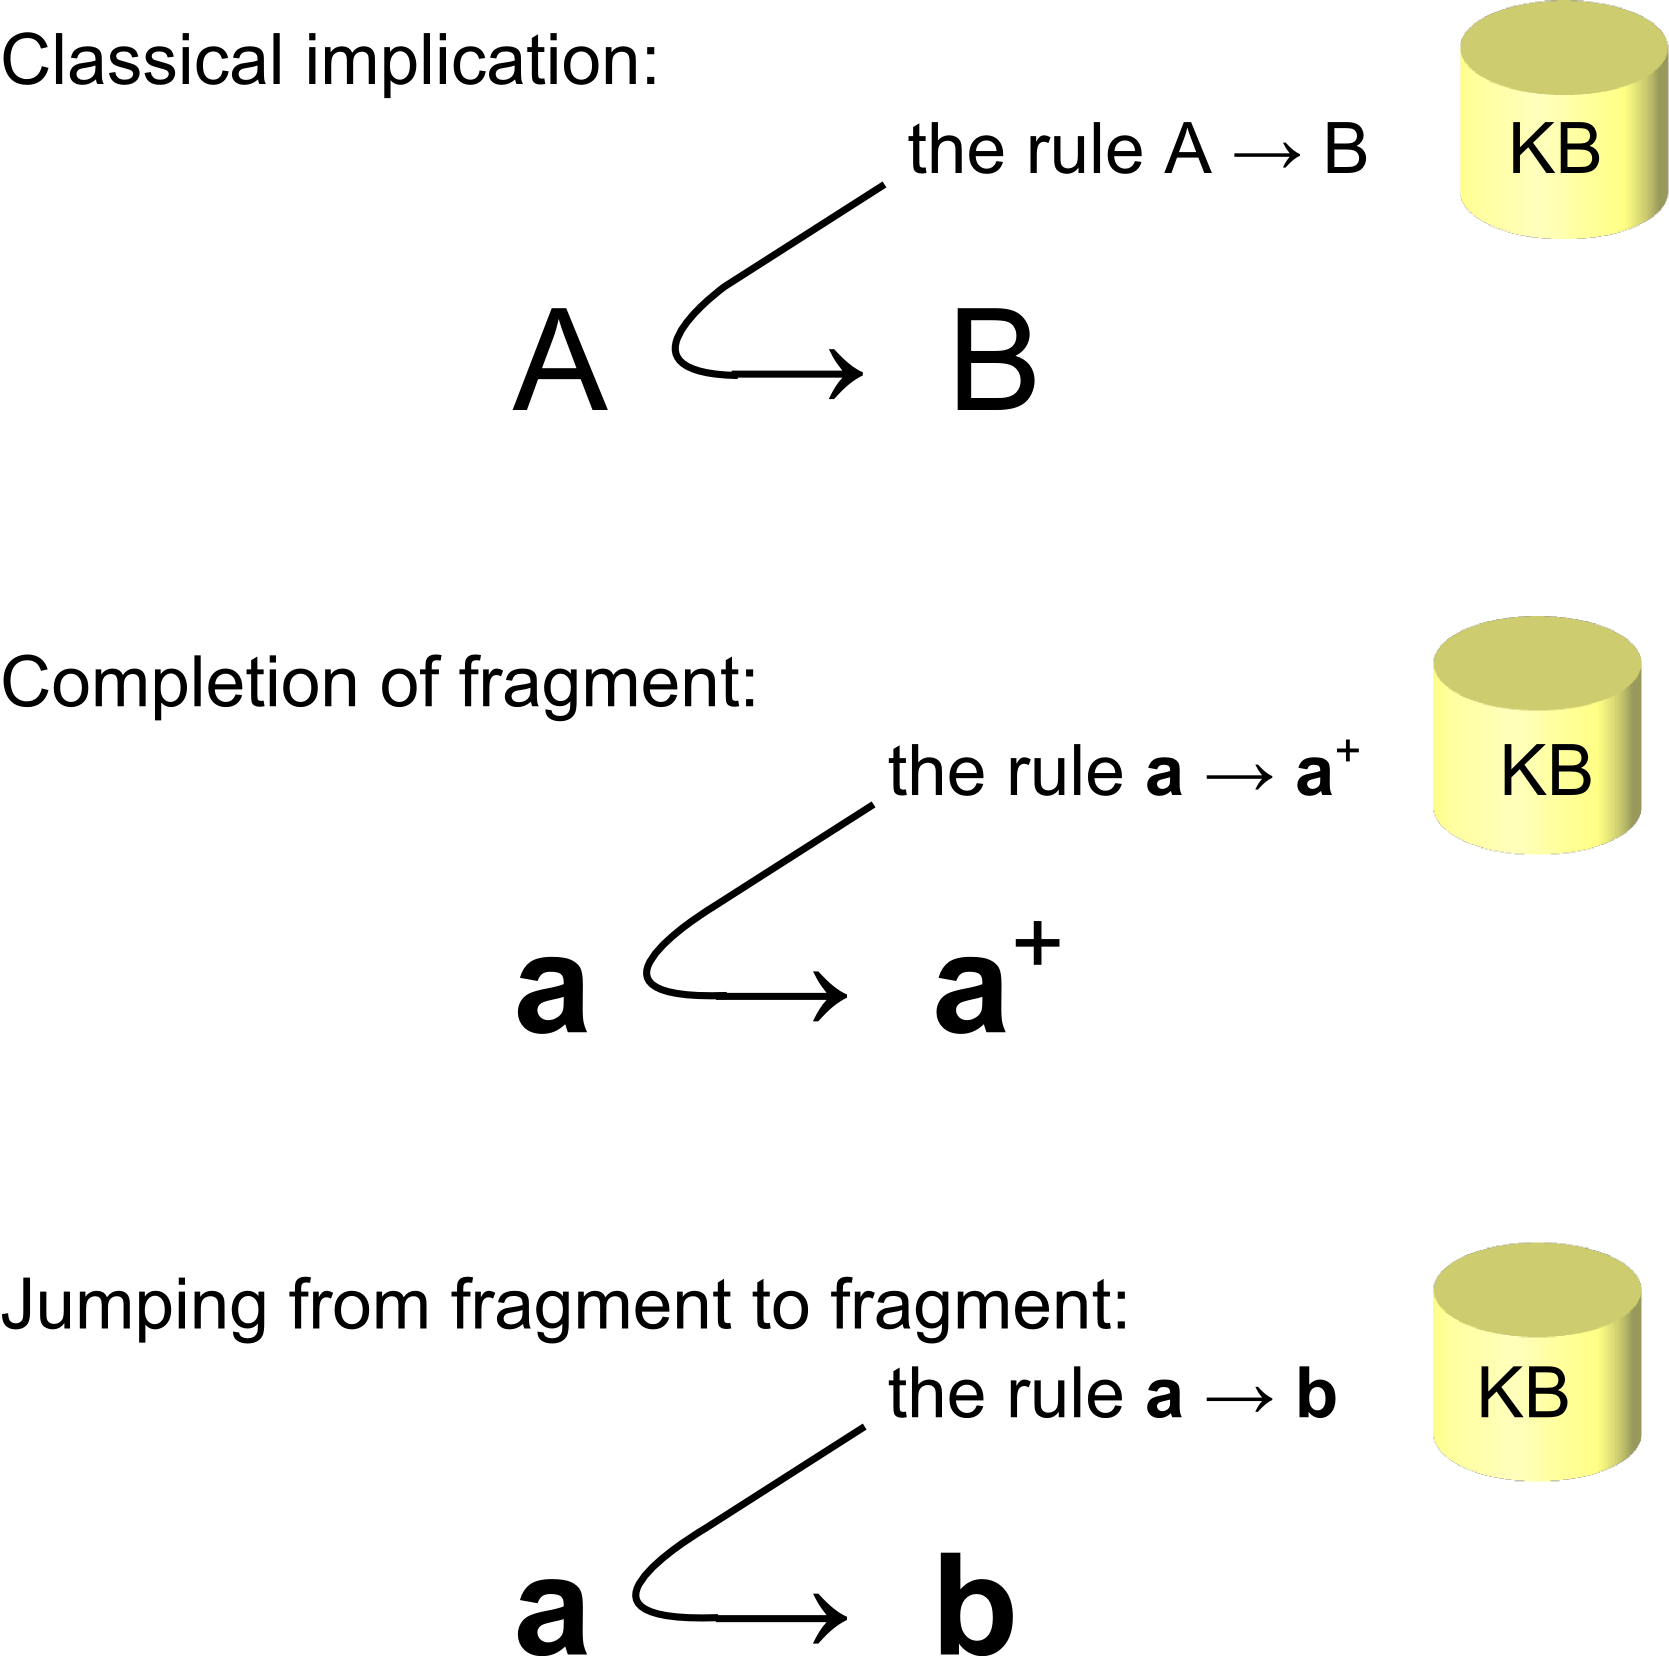
\includegraphics[scale=0.7]{fragments-inference-rules.png}
% \caption{???}
\end{figure}

Note that in all 3 situations, the logic rules are supplied by the KB, which allows an ``arrow'' to be there in the first place.  (The premises are also supplied by the KB, but is not shown in the figure.)  The point is that the conclusions derived from fragments are not arbitrary;  they depend on truths in the KB:  a formula with the generalized arrow is a form of truth;  and the premise fragment is also a form of truth -- it can be interpreted as ``Fragment $\vect{a}$ is worth paying attention to at this moment''.  

Now we can see the symmetry of the 3 forms and that $A \rightarrow B$ can be seen as a special case of $\vect{a} \rightarrow \vect{b}$ (jump).  This leads to the unification of propositional and sub-propositional logic, with a unified ``arrow''.  Thus, our set of logical operators can be minimized to composition ($\circ$, product), union (sum), and exponentiation ($\rightarrow$, arrow).  An interesting question is to see whether the logic can be made a \textbf{CCC} (Cartesian closed category), which seems to be a ``nice'' property to have.

\section{Uncertainty}

Reasoning under uncertainty is a vast and nightmarishly complex topic in AI.  Simon Parsons's book \citep*{Parsons2001} contains a very good survey of uncertain reasoning, but even that is not exhaustive.  We may look at the following taxonomy of ``ignorance'' proposed by \citep*{Bosc1997}:
\begin{figure}[H]
\centering
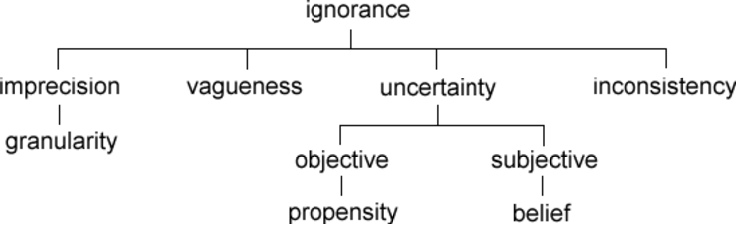
\includegraphics[scale=0.7]{IgnoranceTaxonomy.png}
\caption{taxonomy of ignorance}
\end{figure}

At first blush, classical logic appears to be sufficient for AGI.  Some AGI designers prefer to use crisp logic as the base and plan to build $\mathcal{P}$ and $\mathcal{Z}$ upon crisp logic.  But this may be a sign of not facing problems and not having sufficient understanding of fuzzy-probabilistic logics.  To represent $\mathcal{P}$ and $\mathcal{Z}$ logic \textit{in} crisp logic is like writing an entire $\mathcal{P}$-$\mathcal{Z}$ inference engine in Prolog, complicated by the fact that the crisp logic would be somewhat different from Prolog and so may be even harder to program in.  Also, the ``truths'' known by the AGI will then be different from the truths as represented in the crisp logic --- the former would be ``floating'' above the latter;  This creates unnecessary indirectness.  I will give other reasons in \S\ref{sec:whyZ} and \ref{sec:whyP}.

\textbf{Why not include other uncertainty measures besides $\mathcal{P}$ and $\mathcal{Z}$?}

There are other theories of uncertainty, such as possibility, belief functions, and rough sets.  The reason I chose $\mathcal{P}$ and $\mathcal{Z}$ is because they are simple and best understood.  There has been attempts to create systems where the user can create a flexible number of uncertainty measures, but one problem of such systems has been pointed out in \citep*{Parsons2001}:  If we have 3 uncertainty measures, say ``cloud'', ``mist'', and ``fog'', there would be a need to provide mixed inference rules for ``cloud-mist'', ``cloud-fog'' etc, a total of $n^2$ possibilities.  I have worked out the combination of $\mathcal{B}$, $\mathcal{P}$ and $\mathcal{Z}$ and found that it involved considerable efforts.

\section{Nonmonotonicity and defeasible reasoning}
\label{sec:exceptions}

One can create defeasible logics from classical logic, for example Reiter's \textbf{default logic} and McCarthy's \textbf{circumscription}.  But the classical approaches seem to require enumerating all possible exceptions, which is impractical.

\textbf{2 examples:}

\textbf{A.}\\
\textit{
1. John is usually very punctual.\\
2. Therefore, John will arrive at the airport on time.\\
3. John has an accident en route to the airport, and dies.\\
4. Therefore, John will NOT arrive on time.\\}
Will John arrive on time?

\textbf{B.}\\
\textit{
1. Mary has cybersex with many partners.\\
2. Cybersex is a kind of sex.\\
3. Therefore, Mary has many sex partners.\\
4. A person who has many sex partners has a high chance of STDs.\\
5. Therefore, Mary has a high chance of STDs.}

What's wrong with example B?  On the one hand, we should admit that cybersex is sex (it is a borderline case), but it lacks certain prominent features of sex, such as physical contact (which is not necessarily a \textit{defining} feature of sex).  Thus, if we carry on reasoning with the idea that cybersex is sex, we may get unsound conclusions.  The key to resolving this problem is to recognize ``cybersex is sex'' with \textbf{qualifications} such as ``it is sex without physical contact''.

If we have a rule that ``sex transmits certain diseases'', we may have to attach the exception ``only if the sex involves physical contact''.  In the end, our rules may be inundated with possibly infinitely many exceptions.  How can we get out of this problem?

\citep*{Wang1994}, \citep*{Wang2006} in NARS provided a solution.  His idea is not to store the exceptions to rules, but instead allow a \textit{multitude} of rules to fire, calculate the ``confidence'' (\S\ref{sec:confidence}) of each conclusion, and pick the conclusion with the highest confidence.  This allows us to handle exceptions relatively easily.

For the example:
\begin{eqnarray}
X \PimpL A \nonumber \\
X \PimpL B \nonumber
\end{eqnarray}
Pei Wang's idea is to calculate the combined conditional probability by weighing each individual conditional probability with their associated \textbf{confidences} (\S\ref{sec:confidence}):
$$ P(X|A,B) = \frac{ P(X|A)c_A + P(X|B)c_B }{ c_A + c_B } $$
which is a nice idea\footnote{Except that NARS truth values do not conform to probability theory.}, but Abram Demski came up with an alternative idea that is more in accord with Bayesianism.  The idea is to construct $P(X|A,B)$ from the marginal conditionals $P(X|A)$ and $P(X|B)$ and priors $P(A)$ and $P(B)$.  This is achieved by applying Bayes' rule twice:
\begin{eqnarray}
P(X|A,B) &=& \frac{P(A,B|X)P(X)}{normalization} \nonumber \\
         &=& \frac{P(A|X)P(B|X)P(X)}{normalization} \nonumber \\
         &=& \frac{P(X|A)P(A)P(X|B)P(B)}{P(X) \; normalization}
\end{eqnarray}

It may be possible to use Abram's method to construct all joint CPTs, instead of using contrived probabilistic formulations of AND and OR.

\subsection{An example}

\english{John is usually punctual, therefore, John will arrive at the airport on time.}\\
\english{John died en route to the airport, therefore, John will NOT arrive on time.}

\formula{punctual(john)} = $(P)$ = \tv{0.8} \\
\formula{punctual(john) $\Pimp$ arrive(john)} = $(A \vert P)$ = \tv{0.8} \\
\formula{dead(john) $\Pimp$ arrive(john)} = $(A \vert D)$ = \tv{0.05}

Abram's method:
$$ (A|P,D) = \frac { (A \vert P) (P) (A \vert D) (D) } { (P, D) (A)^{2-1} } $$

\section{Unification}
\label{sec:unification}

Unification is the process of making 2 terms identical via substitutions.  For example, we can use a substitution:
$$ \theta = \{ john/X, mary/Y \} $$
to transform a term like this:
$$ loves(X, Y) \stackrel{\theta}{\longrightarrow} loves(john, mary). $$
Unification ($\bowtie$) is the process of finding the substitution given the initial and final terms.  So:
$$ loves(X, Y) \; \bowtie \; loves(john, mary) = \theta .$$

When we use logic to encode natural language and common-sense reasoning, terms are representations of (simple or compound) \textbf{concepts} (cf \S\ref{sec:composition}).  Thus unification plays the role of deciding if 2 concepts are the same; in other words, the unification algorithm embodies the \textbf{calculus of concepts}.

Two important relations of concepts are:
\begin{enumerate}
\item Equality ($=$).  For example: \formula{clark-kent = superman}.  Can be generalized to fuzzy equality ($\approx$).   For example: \formula{cat $\approx$ dog} (cats are similar to dogs because they are both pet animals).
\item Inclusion ($\subseteq$), in classical AI also known as the "is-a" relation.  For example: \formula{dog $\subseteq$ animal}.
\end{enumerate}

The $=$ relation affects unification because substitution of equals for equals is valid. We use a set of equations, called an equational \textbf{theory}, to define what are considered equal.  Then we have so-called \textbf{unification modulo equational theory}, or \textbf{E-unification}.  The algorithm for equational unification is called \textbf{narrowing}, see \S\ref{sec:narrowing} below.

A complication is that $=$ should be replaced by the more general $\approx$, and we need to modify the traditional algorithms to handle diminishing fuzzy truth values when $\approx$ is repeatedly applied.

\subsection{Higher-order unification}

The standard algorithm for higher-order unification was formulated by Huet in 1974.

\subsubsection{Huet's algorithm}

\underconst

\subsection{Equational unification / narrowing}
\label{sec:narrowing}

\textbf{Narrowing} is \textbf{term rewriting} with \textbf{unification}.  The matching process of rewriting is replaced by unification, where both the rewrite rule and the term to be rewritten can be instantiated.  Some basic texts on narrowing are \citep*{Baader1998}, \citep*{Snyder1991}, \citep*{Prehofer1998}, \citep*{Holldobler1989}.

The equational theory $E$ is replaced by a rewriting system $R$ by \textbf{orienting} the equations in a specific direction.

The \textbf{one-step narrowing relation} $\rewrite{R}$ is induced by a TRS (term rewriting system) $R$.  We write $(t \rewrite{R}^\sigma t')$ to denote a substitution $\sigma$ that enables the term $t$ to be rewritten as $t'$ using \underline{one} rewriting rule from $R$. \\

%The one-step narrowing relation can be extended to equations as:
%$$ (s \approx^?_E t ) \leadsto_R^\sigma (s' \approx^?_E t') $$

\begin{example}
To rewrite:\\
\tab $g(f(a,x))$ \\
when given the equational theory\\
\tab $f(a, h(a)) = c$ \\
we can make the substitution $\{ h(a) / x \}$, yielding:\\
\tab $g(c)$. \\
This step makes the term "narrower", hence the name I guess.
\end{example}

Narrowing is a search process with high complexity because at each step, there are 2 kinds of choices to be made:
\begin{compactenum-}
\item which rewrite rule in $R$ to try; and
\item which position within $t$ to try.
\end{compactenum-}

\section{Equality}
\index{equality}  \index{identity|see{equality}}
\label{sec:equality}

\subsection{Morning star / evening star problem}

A problem with equality is illustrated by the classic example ``Morning Star / Evening Star''.  The following is a similar example with its rendition in logic:

\begin{example}
\label{ex:superman}
\tab
\begin{tabular}{l|l}
\english{Clark Kent is Superman.}            & \formula{clark-kent = superman} \\
\english{Superman can fly.}                  & \formula{can-fly superman} \\
\english{Mary does not know that Clark Kent is Superman.} & $\neg$ \formula{knows(mary, "clark-kent = superman")} \\
\english{Mary knows that Superman can fly.}  & \formula{knows(mary, can-fly superman)} \\
\english{Mary does not know that Clark Kent can fly.} & $\neg$ \formula{knows(mary, "can-fly clark-kent")}
\end{tabular}
\end{example}

A possible solution is to distinguish \formula{"clark-kent"} (in quotes, ie, the Clark Kent that Mary knows) and \formula{clark-kent} (without quotes, ie, the real Clark Kent).  This idea is similar to the so-called "use / mention" distinction:\\
\tab \begin{tabular}{ll}
\textbf{Use:}      & Cheese is derived from milk.\\
\textbf{Mention:}  & ``Cheese'' is derived from the old-English word ``cyse''.
\end{tabular}

%\begin{example}[\english{John thinks that he can fly.}]
%We can render this in logical form (\S\ref{sec:geniform}):\\
%\tab \formula{\kb{1} s$_2$ that thinks john}\\
%\tab \formula{\kb{2} can-fly john} \quad \tv{with indefinite TV}\\
%\tab \formula{\kb{3} can-fly john} \quad \tv{with low probability}\\
%where s$_3$ is a fact we assume the agent already knows in its KB.  The agent will assign an indefinite fuzzy truth value (ie, a uniform probability distribution over $[0,1]$) to s$_2$, since it is a quoted statement.  This requires the ability to store  multiple copies of syntactically identical statements.
%\end{example}

The problem is in general due to the presence of ``contexts'' (cf \S\ref{sec:contexts}).  For example
\begin{compactitem-}
\item In the context of children's tales, animals can talk.
\item In the context of Star Wars, Darth Vader is Luke's father.
\item In the context of Mary's beliefs, Superman and Kent are different persons.
\end{compactitem-}

\section{Modal logic}
\begin{flushright}
\emph{Modality, si! Modal logic, no!}\\
--- John McCarthy
\end{flushright}

My view is to use predicates to represent modality instead of using modal logics.  This view was first advocated by \citep*{McCarthy1997}.

One argument for the use of modal logic arises from the previous Example \ref{ex:superman}:\\
\begin{tabular}{l|l}
\tab \english{Mary knows Superman can fly.} & \formula{knows(mary, can-fly superman)}\\
\tab \english{Superman is Clark Kent.} & \formula{superman = clark-ken}\\
\hspace*{0.7cm} * \english{Mary knows Clark Kent can fly.} & \formula{knows(mary, can-fly clark-ken)}
\end{tabular}\\
but Mary may not know that Superman is Clark Kent.  This problem can be resolved as in the last section (\S\ref{sec:equality}).

\section{Logical paradoxes}
\label{sec:paradox}

\underconst

\subsection{Russell's or Liar's paradox.}

\subsection{Curry's paradox.}

\subsection{Skolem's paradox.}

\subsection{Tarski's paradox.}

\subsection{Non-axiomatizability.}

``First order logic has an effective notion of proof which is complete w.r.t. the intended interpretation.  This is the content of Godel's completeness theorem.  As a result, the set of (Godel numbers of) universally valid first-order formulas is recursively enumerable.''  But ``the set of second order validities is not arithmetically definable let alone recursively enumerable and hence that an effective and complete axiomatization of second-order validity is impossible'' \citep*{Benthem}.

\section{Shortcomings of the current logic}

\textbf{Binary vs $\mathcal{P/Z}$.}  It may be desirable to have binary logic alongside $\mathcal{P/Z}$ logic.  $\mathcal{P/Z}$ reasoning is suitable for common-sense concepts, whereas binary reasoning is good for \textit{programmatic}
\footnote{Ie, binary logic makes programming easier}
or computational reasons.  However, one unsolved problem is that many common-sense concepts appear to be binary but are fuzzy upon close inspection (eg male/female, dead/alive).  The question is how to let binary and fuzzy concepts coexist in the same logic.

%\section{$\mathcal{B}$: binary logic}
%\label{sec:binary-logic}

%My intuition is that common-sense reasoning involves mainly $\mathcal{B}$, followed by $\mathcal{Z}$, and $\mathcal{P}$ is relatively rare.

%Horn clauses:  P and Z rules can be expressed in Horn form only.  But it seems that we can use general resolution for B rules, no?  Or, perhaps I want to use something similar to Horn resolution for P and Z?

%Each rule will enable one inference step, so the logic is almost truth-functional.  The problem is the intermediate results... I only know how to do that in B form.  Maybe we can keep a set of disjunctions of truth values?

%In B logic the proof procedure keeps a current clause / or a line of clauses.  In Bayes net we have a query variable and the algorithm finds its P value.  Z logic may be similar to B logic because it's truth functional?

%Perhaps we can work out the general case of a query variable of any TV type?  If we draw a B rule that's easy.  If Z rule, then we have a few Z variables as goals.  They need Z rules to fulfill, but what if we have a B rule for one of the sub-goals?  Then we need to translate the B value to Z value.  We can only do that via P(Z).  So we have a P(Z) value as one of the subgoals.  This may cause the head of the rule to become P(Z) too.  It seems there is a tendency for all TVs to become P(Z).
%That will actually back-propagate along the proof sequence.

%Things may be even worse for a P rule.  The application of the rule requires other numbers.  

\section{Meta-reasoning}
\begin{flushright}
\emph{I think I think, therefore I think I am.}
\end{flushright}

The term ``meta-reasoning'' may refer to 2 things:\\
1. The ability to \textbf{reason about reasoning}, which is what this chapter is concerned with;\\
2. Scheduling reasoning tasks to achieve best results with limited computational resources (I have not thought about this problem yet).

An excellent survey of meta-reasoning in the \#1 sense is \citep*{Constantini2002}.

In the Tell-Learn loop, we see that we need a special predicate credible() to increase the probability of a statement via a side-effect.  But that may not be the only meta-reasoning move we can make.

Another example is the $B \leftrightarrow Z$ conversion of ``traitor'' and ``patriot'' (\S\ref{sec:PZ-meta-reasoning}).

\section{Higher order logic}
\label{sec:HOL}

\citep*{Lloyd2003} developed inductive learning based on HOL, a \textbf{typed lambda calculus}, and also a logic programming language (Escher).

Lloyd uses a form of logic that is similar to what I do with $\mathcal{P(Z)C}$ logic, ie, its statements are of the form $H = B$ where $H$ is the head and $B$ is the body.  In essence this is the Prolog / Horn tradition.

\{ TO-DO:  formulate a $\mathcal{P(Z)C}$ HOL \}

\label{sec:PZ-meta-reasoning}

One example of meta-reasoning pertinent to fuzziness is:\\
\hspace*{1cm} S1: ``You are either a patriot or a traitor.''\\
\hspace*{1cm} S2: ``No, I can be slightly patriotic or slightly traitorous.''

In S1 the predicates \textit{patriot} and \textit{traitor} have binary character.  In S2 they have fuzzy character.

\underconst

\section{Algebraic logic}

My motivation for studying algebraic logic is to develop better inference and learning algorithms for logic.  In the 1990s, the invention of SVMs by Vapnik revolutionized the field of statistical learning, and SVMs remain to be the best general spatial learner today.  What if we can invent something similar to logic as what SVM is to spatial domains?

\subsection{Survey of algebraic logic}

\citep*{Halmos1962}, \citep*{Andreka2001}, \citep*{Halmos1988}, \citep*{Craig1974}, \citep*{Plotkin1994}, \citep*{Lawvere2003}'s Appendix A.

\todo{Lawvere's idea that the existential and universal quantifiers are adjuncts to each other.  What use is it?}

\subsection{Speeding up inference and learning}

For all logics that I know of, deduction is performed by \textit{iterating} deductive steps.  Each step is the application of an inference rule.  If a formula with quantification is involved, some kind of pattern matching or unification is required apply the formula.  Such an iterative process is equivalent to searching in a large proof space.

My idea is:  perhaps we can ``map'' logic to some \textit{continuous} space, and somehow approximate the proof process by spatial computational techniques?

One natural idea is:

\tab \begin{tabular}{rll}
first-order objects & $\longrightarrow$ & points in space\\
predicates          & $\longrightarrow$ & regions / shapes in space\\
logical entailment  & $\longrightarrow$ & finding intersections of regions\\
\end{tabular}

\begin{figure}[H]
\centering
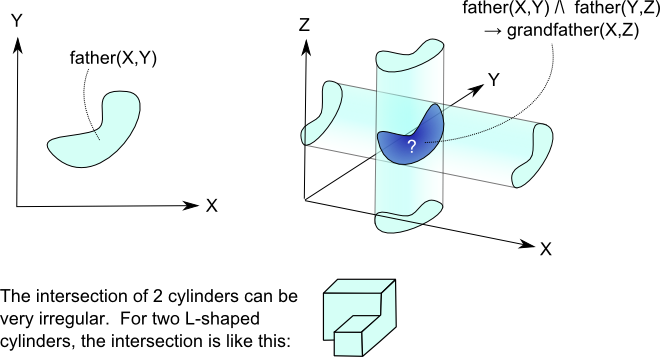
\includegraphics[scale=1.0]{cylindrical-logic.png}
%\caption{algebraic logic}
\end{figure}

We know that, for some concepts (predicates), the shape of the regions defining the predicate can be extremely irregular or even incomputable.

Our motivation is twofold:\\
1. How can we find intersections of regions efficiently?\\
2. Can we altogether avoid performing deduction via iterative steps?

One idea is to have multiple ``domain grids''.  We'd be sorting the source domains into various clusters.  That will speeed up the look-up of intersections.

However, this idea only gives us a geometric interpretation, but it doesn't tell us how to compute the shapes of regions efficiently.  The only way to compute the regions is to go back to the basic inference rules of the logic, ie, iteratively and syntactically.

Another idea is the ``dual'':

\tab \begin{tabular}{rll}
first-order objects & $\longrightarrow$ & shapes / regions in space\\
predicates          & $\longrightarrow$ & points in space\\
logical entailment  & $\longrightarrow$ & ?\\
\end{tabular}
